\chapter{Sistema de información}
\section{Introducción}

Las nuevas tecnologías de análisis genético son fáciles y económicas de hacer lo que genera una gran cantidad de datos biológicos y lo que hace que los biólogos trabajen cada vez más con las nuevas tecnologías de análisis genético, haciendo que los biólogos trabajen más y más computacionalmente.Especialmente mediante el uso de  tecnologías de secuenciación (NGS) y presentar un reto para integrar y almacenar la información, pasos que son necesarios para su posterior análisis \cite{Li2014,Cook2016}.\\

La gran cantidad de datos presentan un reto para organizar y manejar datos que crecen de manera exponencial y que son de diversos tipos, dado que los datos son generados a diferentes niveles y con diferentes métodos (ejemplo: Variantes de exones o imágenes de patología), datos que a su vez deben ser almacenados en distintas formas, esta situación muestra una seria dificultad para realizar un análisis integral de los datos \cite{Cook2016,Li2014}.\\

El mayor de los retos es crear herramientas que permitan al investigador acceder a la información fácilmente y que pueda tener una base de datos intercalable,donde pueda consultar, analizar y actualizar la información de sus experimentos \cite{Li2014}.\\

En el campo clínico esto representa un reto aun mayor dado que se hace necesario recolectar los datos genéticos junto con los datos clínicos para poder hacer análisis más acertados y a gran escala \cite{Paila2013}.\\

El problema de la heterogeneidad  de los datos  se aplica igualmente a los datos clínicos que describen pacientes individuales y además a los datos biológicos que caracterizan nuestro genoma. Específicamente, las bases de datos son altamente heterogéneas con respecto a los modelos de datos que emplean, los esquemas de datos que especifican, los lenguajes de consulta que soportan y las terminologías que reconocen \cite{Sujansky2001}.\\

Por ello se hace necesario que se utilicen herramientas para la gestión de la información, por ejemplo django que es un web framework de alto nivel desarrollado en python  fomenta el desarrollo rápido y limpio, para la creación de aplicaciones web, es de código abierto y gratuito.Se basa en los principios de desarrollo rápido, manejo de la seguridad y es altamente escalable . Dentro de las muchas aplicaciones que tiene django una es el manejo y gestión de bases de datos a través de los módulos de python. Ver documentación https://www.djangoproject.com/ \\.


\section{Metodología}

Nosotros a continuación proponemos la utilización de una base de datos con la información clínica disponible y las anotaciones de variantes obtenidas por medio de un pipeline validado previamente para la anotación de variantes, basado en la propuesta de Fisch y colaboradores en 2014 \cite{Fisch2015} y anotados con annovar web service \cite{Yang2015}. Las historias clinicas fueron transcritas manualmente y cargadas desde un archivo de texto plano con un formato especifico.\\

Se genero una base de datos utilizando Django 1.10 en python 3 y la librería grapelli, que se conectan  a  MySQL  5.7.17 desde un PC portatil HP-pavilion 360 con ubuntu 16.04 LTS. Django genera los modelos de EER pero permite su modificación para optimizar la velocidad de las consultas. \\

\section{Resultados} 

Los resultados obtenidos fueron una aplicación con una interfaz que permite a los usuarios con poco conocimiento de  programación  analizar los datos de variantes y su resumen de la historia clínica. \\

\begin{figure}[h] 
	\centering
	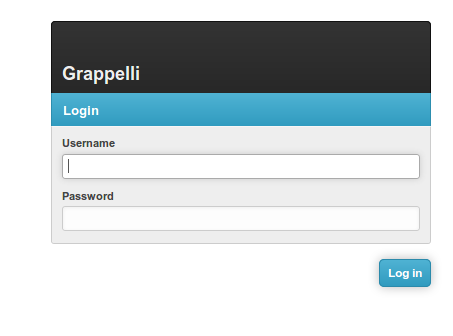
\includegraphics[width=0.4\textwidth]{Kap3/admin_django}
	\caption{Interfaz de ingreso para  administrar la base de datos.} \label{fig:admin}
\end{figure}

Inicialmente la figura (\ref{fig:admin}), muestra la solicitud de usuario y contraseña para acceder a la aplicación, es diferente a la base de MySQL que puede tener  una contraseña igual o diferente a la interfaz gráfica .

\begin{figure}[h] 
	\centering
	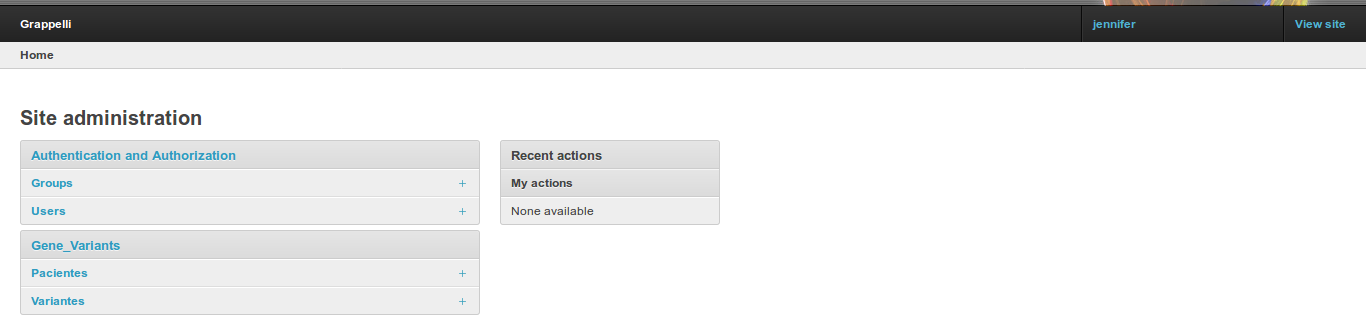
\includegraphics[width=0.5\textwidth]{Kap3/django_admin}
	\caption{Interfaz de administración.} \label{fig:admin2}
\end{figure}

La figura (\ref{fig:admin2}), muestra el sitio de administración donde se encuentran los usuarios permitidos, las bases de datos a consultar y muestra un histórico de las actividades recientes. \\

Desde esta interfaz se puede agregar un grupo, más usuarios y pacientes y/o variantes dando click en el signo más sin necesidad de hacer la carga directa a MySQL ya que Django se encarga de hacer la carga. \\

\begin{figure}[h] 
	\centering
	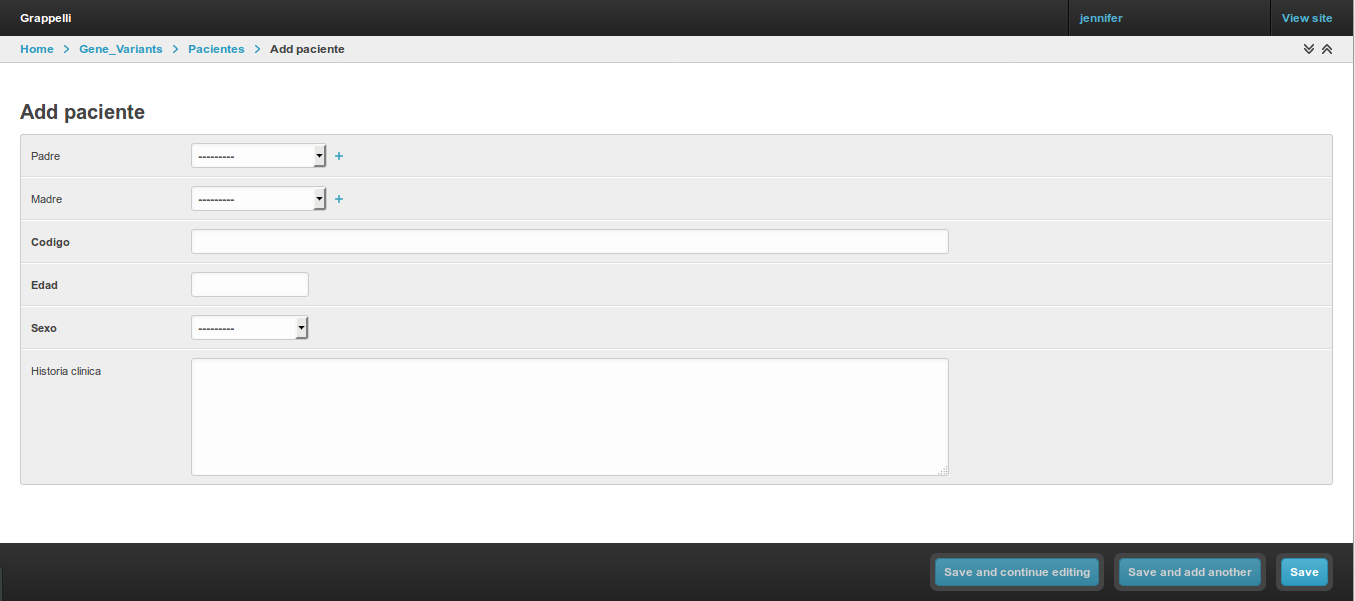
\includegraphics[width=0.5\textwidth]{Kap3/ingresar_paciente}
	\caption{Ingreso de pacientes.} \label{fig:pacientes}
\end{figure}

En la figura (\ref{fig:pacientes}) se muestra el formulario para ingresar una nueva historia o de modificar una historia clínica de un paciente de manera manual.

\begin{figure}[h] 
	\centering
	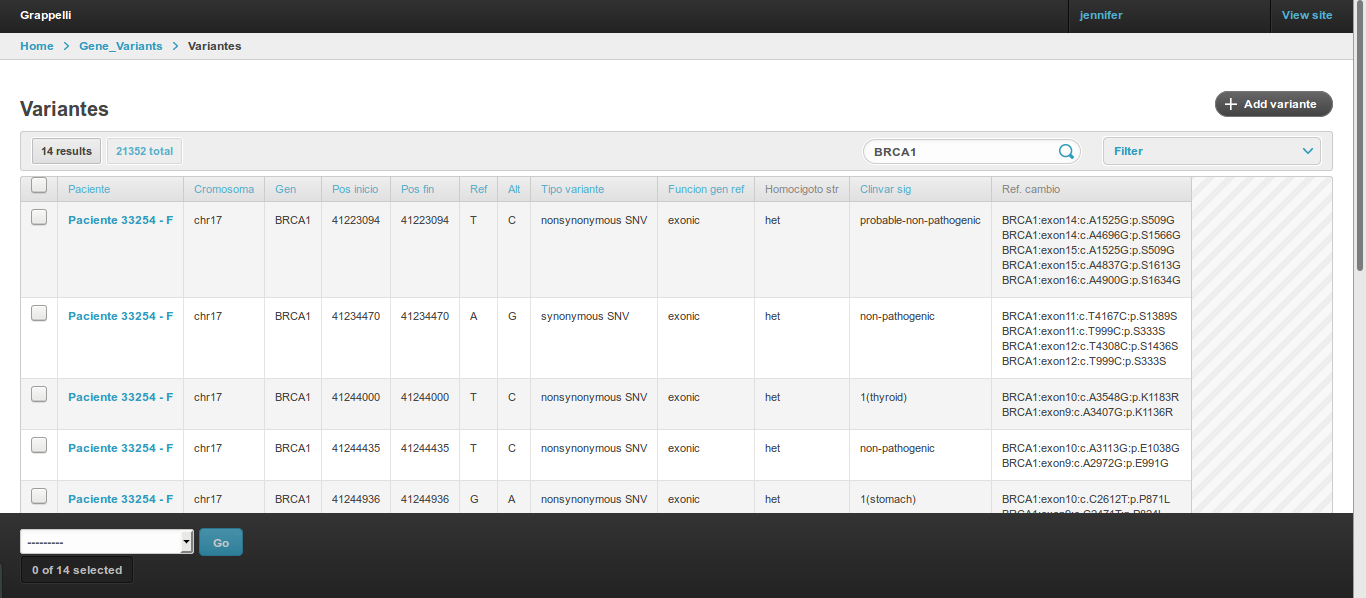
\includegraphics[width=0.5\textwidth]{Kap3/consulta}
	\caption{Consulta a variantes} \label{fig:consulta}
\end{figure}


La figura (\ref{fig:consulta}) muestra una consulta de las variantes que se tienen cargadas en la base de datos para el gen BRCA1, donde nos muestra una consulta de las variantes con su anotación  filtrada mediante un script de python antes de cargar las anotaciones de la tabla obtenida por annovar para cada paciente. Desde esta misma interfaz se puede hacer consultas de pacientes que se deben eliminar, en la parte inferior se encuentra la opción.\\

Si se desea hacer modificaciones a los datos del paciente también es posible hacerlo desde esta misma interfaz seleccionando el código del paciente, que lleva a la tabla de genes\_varante\_paciente que contiene el formulario de la historia clínica con los datos cargados para ser modificados. 

\begin{figure}[h]
	\centering
	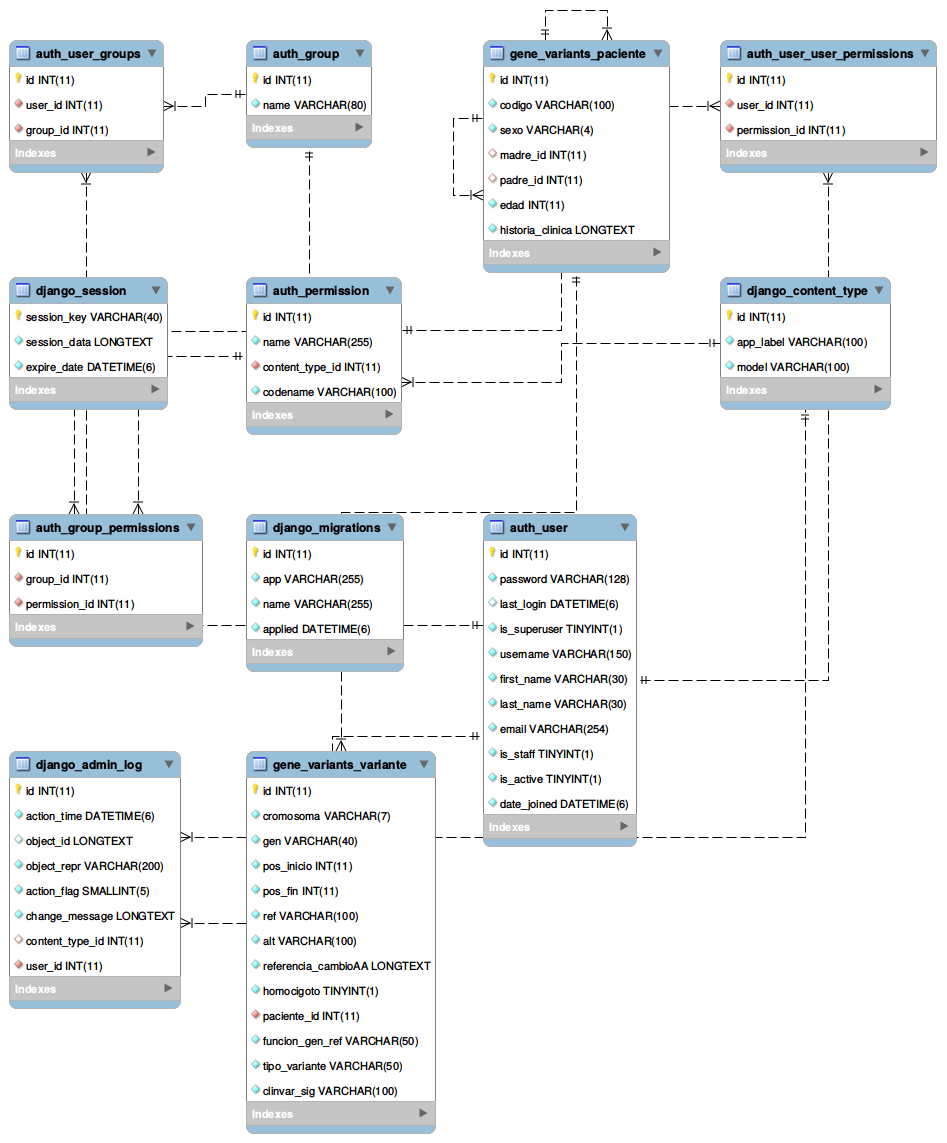
\includegraphics[width=0.8\textwidth]{Kap3/modeloEER}
	\caption{Modelo entidad relación} \label{fig:t}
\end{figure}

La figura (\ref{fig:t}) muestra el modelo EER que se genero en la base de datos MySQL, donde se muestra el modelo  EER que muestra las tablas generadas por la aplicación para crear la base de datos donde se incluyen las tablas de para la gestión del las variantes junto con la historia clínica y se tiene encuentra la posible relación parental, padre, madre e hijo, el control de las consultas de la variantes indexadas y dentro de la misma base la gestión de accesos a otros usuarios con sus permisos.

\section{Discusión}
\subsection{Gestión de datos biológicos}

La importancia de gestión aplicada al manejo de datos clínicos y de información genética es de vital importancia dado que existen miles de anotaciones que requieren de scripts para cargarlos las anotaciones y como es este caso el historial clínico del paciente \cite{Paila2013}. \\

La aplicación desarrollada para crear y gestionar una base de datos aplicada una bioinformática con aplicaciones a la medicina, es necesario que la base de datos provea las consultas para soportar las decisiones sobre un paciente en especifico teniendo en cuenta sus datos,la relación con datos de otros pacientes y los datos de exomas, además de los datos relacionados con los familiares en caso de que se encuentren estos datos. Mostrando que es posible realizar una integración adecuada de los datos bioinformáticos y clínicos utilizando bases de datos relacionales, con una buena respuesta en las consultas. \cite{Sujansky2001}.

\section{Conclusión}
La utilización de aplicaciones en Django permite que un bioinformático diseñe e implemente bases de datos aplicadas al diagnostico clínico, donde se puede guardar y gestionar toda la información obtenida de un paciente, lo que permite hacer análisis a profesionales Médicos y biólogos fácilmente. Una vez ha sido implementa la base de datos también es posible aplicar técnicas de minería de datos para optimizar los análisis  de los pacientes. \\